\documentclass[11pt,letterpaper,boxed]{pset}

\usepackage[margin=0.75in]{geometry}
\usepackage{ulem}

\begin{document}

    \problemlist{PHYS051 HW11}
    \begin{center}
        P38.11, *E38.14, E38.16, P38.13, E38.42
    \end{center}
    
    \begin{problem} [P38.11]
        A coaxial cable (inner radius $a$, outer radius $b$) is used as a transmission line between a battery $\mathscr{E}$ and a resistor $R$, as  shown in Fig. 38-28. 
        
        \begin{enumerate}
            \item [a.] Calculate $E, B$ for $a < r < b$.
            \item [b.] Calculate the Poynting vector $\Vec{S}$ for $a < r < b$.
            \item [c.] By suitably integrating the Poynting vector, show that the total power flowing across the annular cross section $a < r < b$ is $\mathscr{E}^2/R$. Is this reasonable?
            \item [d.] Show that the direction of $\Vec{S}$ is always from the battery to the resistor, no matter which way the battery is connected.
        \end{enumerate}
    \end{problem}
    
    \begin{figure*} [ht]
        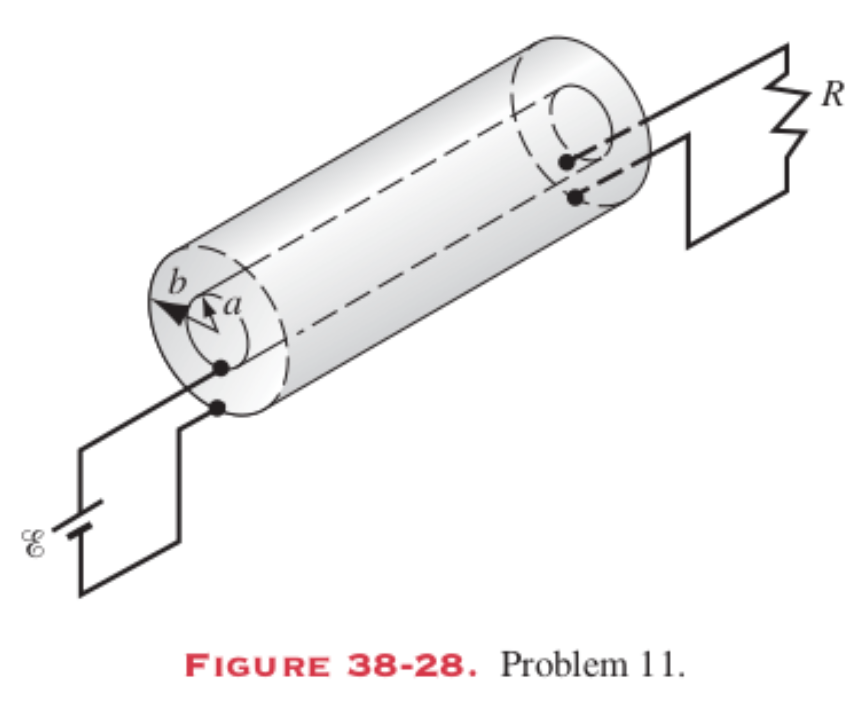
\includegraphics[width = 125px]{HW11Images/P38-11.png}
        \label{fig:P38-11}
    \end{figure*}
    \newpage
    
    \begin{problem} [*E38.14]
        Figure 38-21 shows an $LC$ oscillator connected by a transmission line to an antenna of a magnetic dipole type. Compare with Fig. 38-5, which shows a similar arrangement but with an electric dipole type of antenna. 
        
        \begin{enumerate}
            \item [a.] What is the basis for the names of these two antenna types?
            \item [b.] Draw figures corresponding to Figs. 38-6 and 38-7 to describe the electromagnetic wave that sweeps past the observer point $P$ in Fig. 38-21. 
        \end{enumerate}
    \end{problem}
    
    \begin{figure} [ht]
        \centering
        \begin{minipage}{0.7\textwidth}
            \centering
            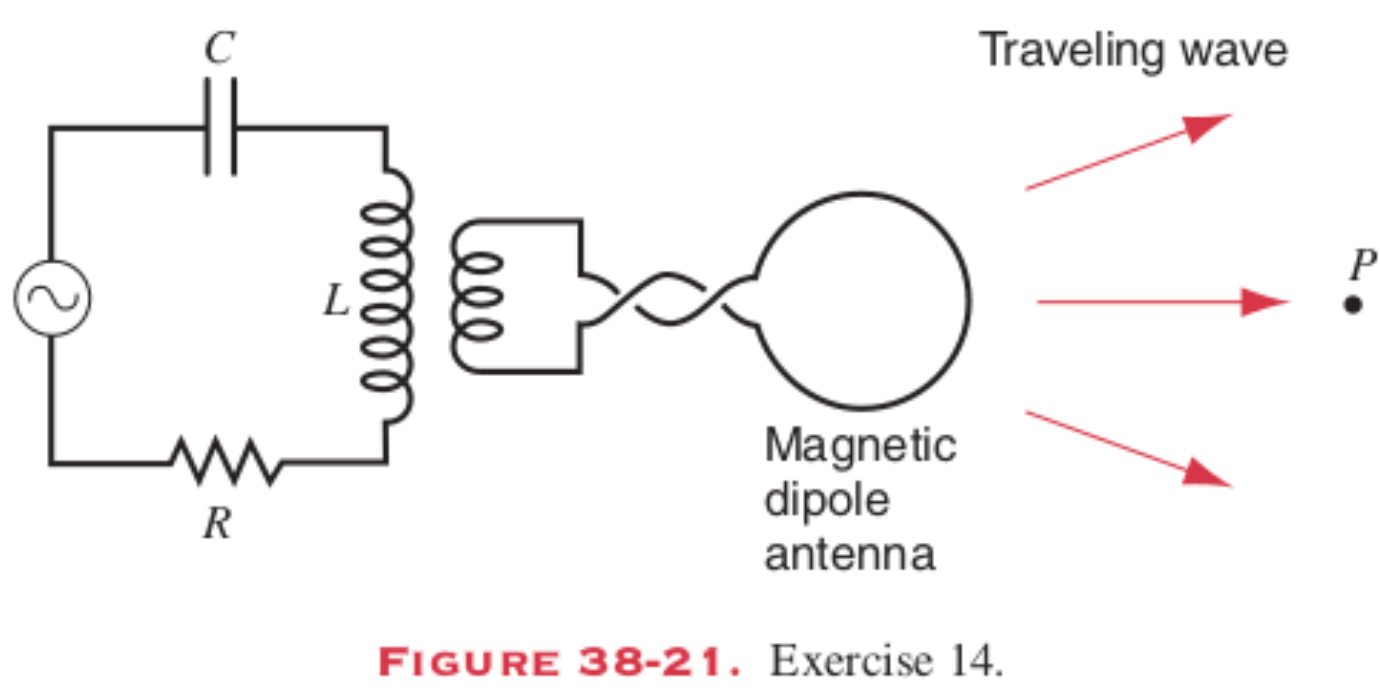
\includegraphics[width=0.45\textwidth]{HW11Images/E38-14.png}
            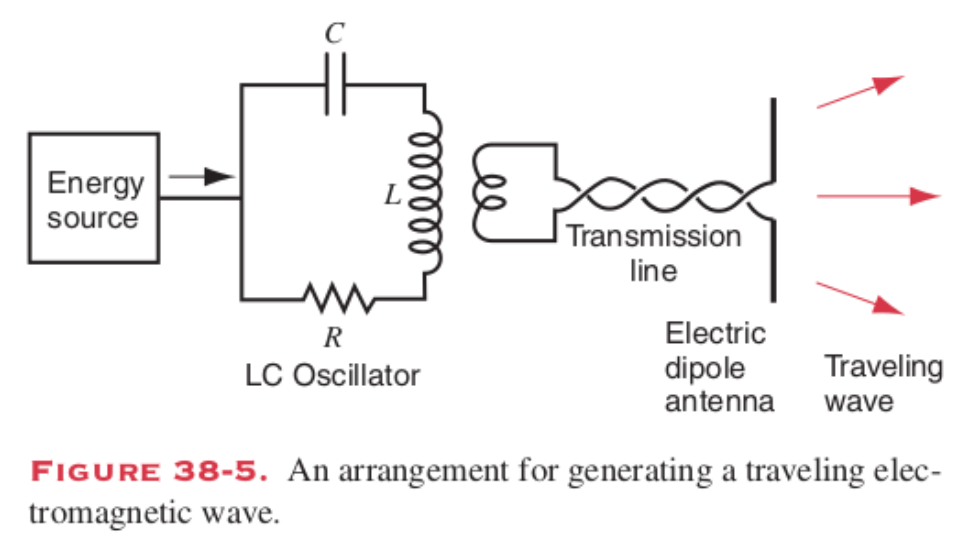
\includegraphics[width=0.45\textwidth]{HW11Images/Fig38-5.png}
            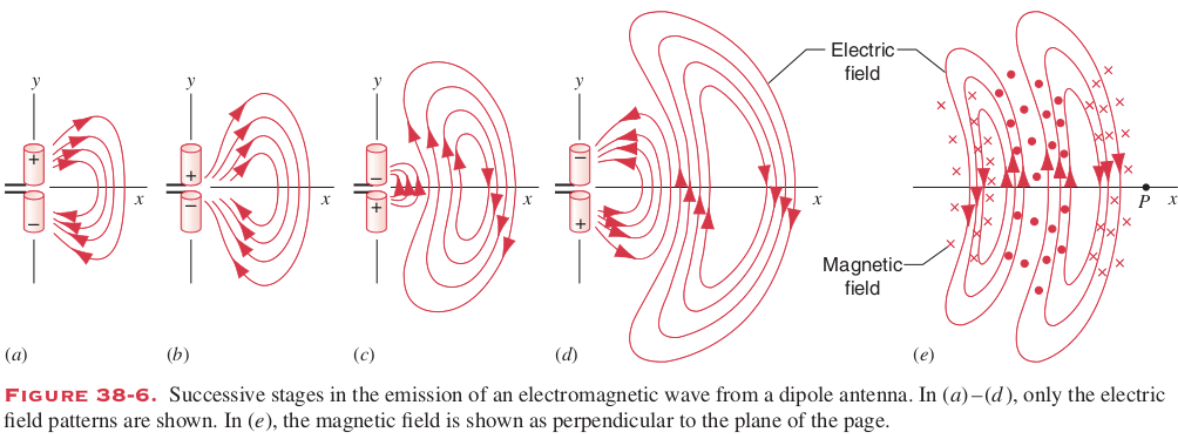
\includegraphics[width=0.85\textwidth]{HW11Images/Fig38-6.png}
        \end{minipage}
        \begin{minipage}{0.25\textwidth}
        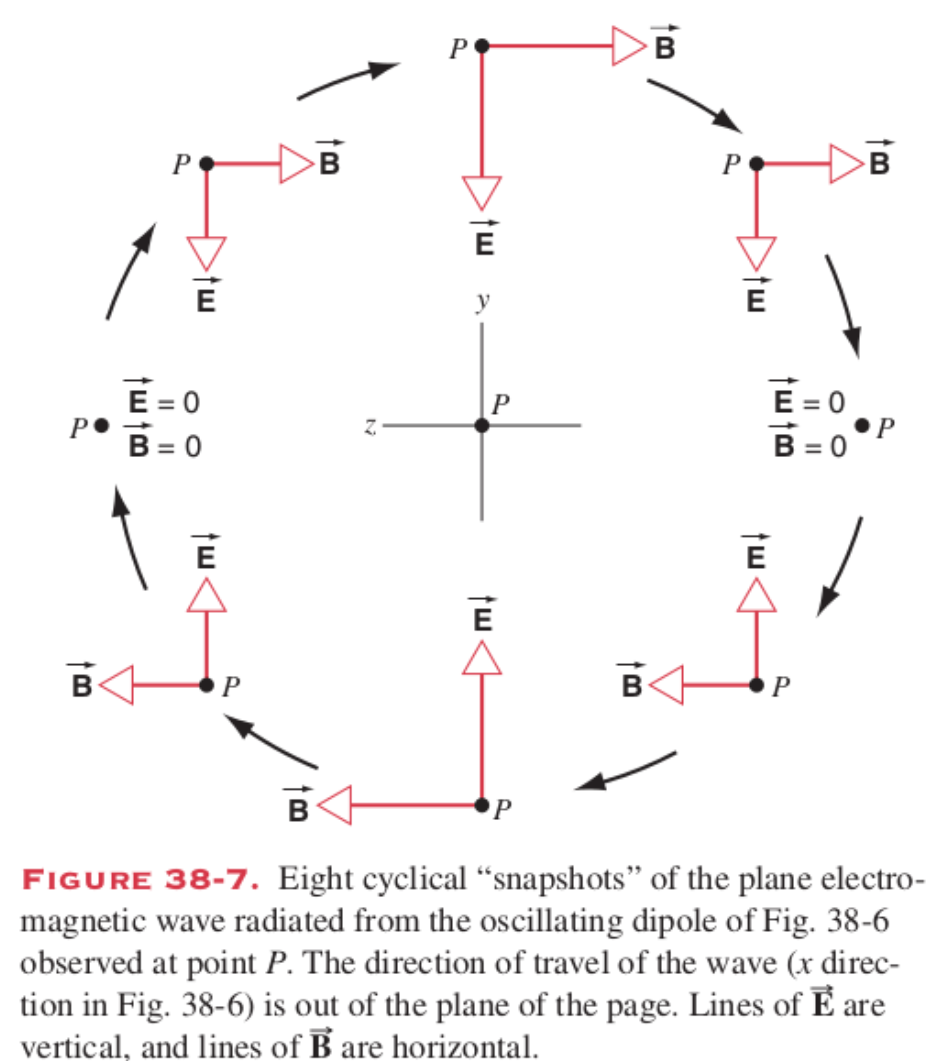
\includegraphics[width=\textwidth]{HW11Images/Fig38-7.png}
        \end{minipage}
    \end{figure}
    \newpage
    
    \begin{problem} [E38.16]
        The electric field associated with a plane electromagnetic wave is given by $E_x = 0, E_y = 0, E_z = E_0 \text{sin} k(x-ct),$ where $E_0 = 2.34 \times 10^{-4}$ V/m and $k = 9.72 \times 10^6$ m$^{-1}$. The wave is propagating in the $+x$ direction. 
        
        \begin{enumerate}
            \item [a.] Write the expressions for the components of the magnetic field of the wave.
            \item [b.] Find the wavelength of the wave.
            \item [c.] What is the wave’s frequency and what kind of radiation is it? \textit{(See Ch. 39 for a hint.)}
        \end{enumerate}
    \end{problem}
    \newpage
    
    \begin{problem} [P38.13]
        A plane electromagnetic wave, with wavelength 3.18 m, travels in free space in the $+x$ direction with its electric vector $\Vec{E}$, of amplitude 288 V/m, directed along the $y$ axis.
        
        \begin{enumerate}
            \item [a.] What is the frequency of the wave?
            \item [b.] What is the direction and amplitude of the magnetic field associated with the wave?
            \item [c.] If $E = E_m \text{sin} (kx - \omega t)$, what are the values of $k$ and $\omega$?
            \item [d.] Find the intensity of the wave.
            \item [e.] If the wave falls on a perfectly absorbing sheet of area 1.85 m$^2$, at what rate would momentum be delivered to the sheet and what is the radiation pressure exerted on the sheet?
        \end{enumerate}
    \end{problem}
    \newpage
    
    \begin{problem} [E38.42]
        A small spaceship whose mass, with occupant, is 1500 kg is drifting in outer space, where the gravitational field is negligible. If the astronaut turns on a 10.0-kW laser beam, what speed would the ship attain in one day because of the reaction force associated with the momentum carried away by the beam?
    \end{problem}
    \newpage
\end{document}